
%使用XeLaTeX编译
%版权所有,翻版必究
%本文件由程序自动生成,任何修改将被覆盖
%2019 年 01 月 23 日




\FloatBarrier
\section{
扫雷
}\label{s100810t05}


最后,举一个稍微复杂一点的小例子:实现一个简单的扫雷程序。

项目目录结构如\treeindexnumbernameone\ \ref{d000003}所
示。

%\begin{spacing}{1.0}
%\FloatBarrier
\refstepcounter{treeindexnumber}\label{d000003}    %增加目录树编号
\begin{thebookfilesourceonepathtree}[escapeinside={(*@}{@*)},
caption=GoodLuck,
numbers=none,
title=\treeindexnumbernameone \thetreeindexnumber
]
.
├── minesweeping.pro
├── main.cpp
├── MineSweepingLine.cpp
├── MineSweepingLine.hpp
├── MineSweepingLineNode.cpp
├── MineSweepingLineNode.hpp
├── MineSweeping.hpp
├── MineSweeping.cpp
└── myqml
    ├── minesweeping
    │   ├── Boom.qml
    │   ├── Error.qml
    │   ├── Flag.qml
    │   ├── Mine.png
    │   ├── Mine.qml
    │   ├── MineMenuBar.qml
    │   ├── MineResetDialog.qml
    │   ├── Number.qml
    │   ├── OkMine.qml
    │   ├── Win.qml
    │   └── main.qml
    └── minesweeping_qtquickcontrols2.conf(*@\marginpar[\hfill\setlength\fboxsep{2pt}\fbox{\footnotesize{\kaishu\parbox{1em}{\setlength{\baselineskip}{2pt}\treeindexnumbernameone}}\footnotesize{\thetreeindexnumber}}]{\setlength\fboxsep{2pt}\fbox{\footnotesize{\kaishu\parbox{1em}{\setlength{\baselineskip}{2pt}\treeindexnumbernameone}}\footnotesize{\thetreeindexnumber}}}@*)\end{thebookfilesourceonepathtree}          %抄录环境
\addtocounter{lstlisting}{-1}   %sub lstlisting counter ...
%\end{spacing}


此项目运行效果
如\figurename\ \ref{p000065}所
示。

%begin图片
\begin{figure}[htb] %浮动体 here and top ...
%there must use marginnote ...
\marginnote{\setlength\fboxsep{2pt}\fbox{\footnotesize{\kaishu\figurename\,}\footnotesize{\ref{p000065}}}}\centering %中心对齐
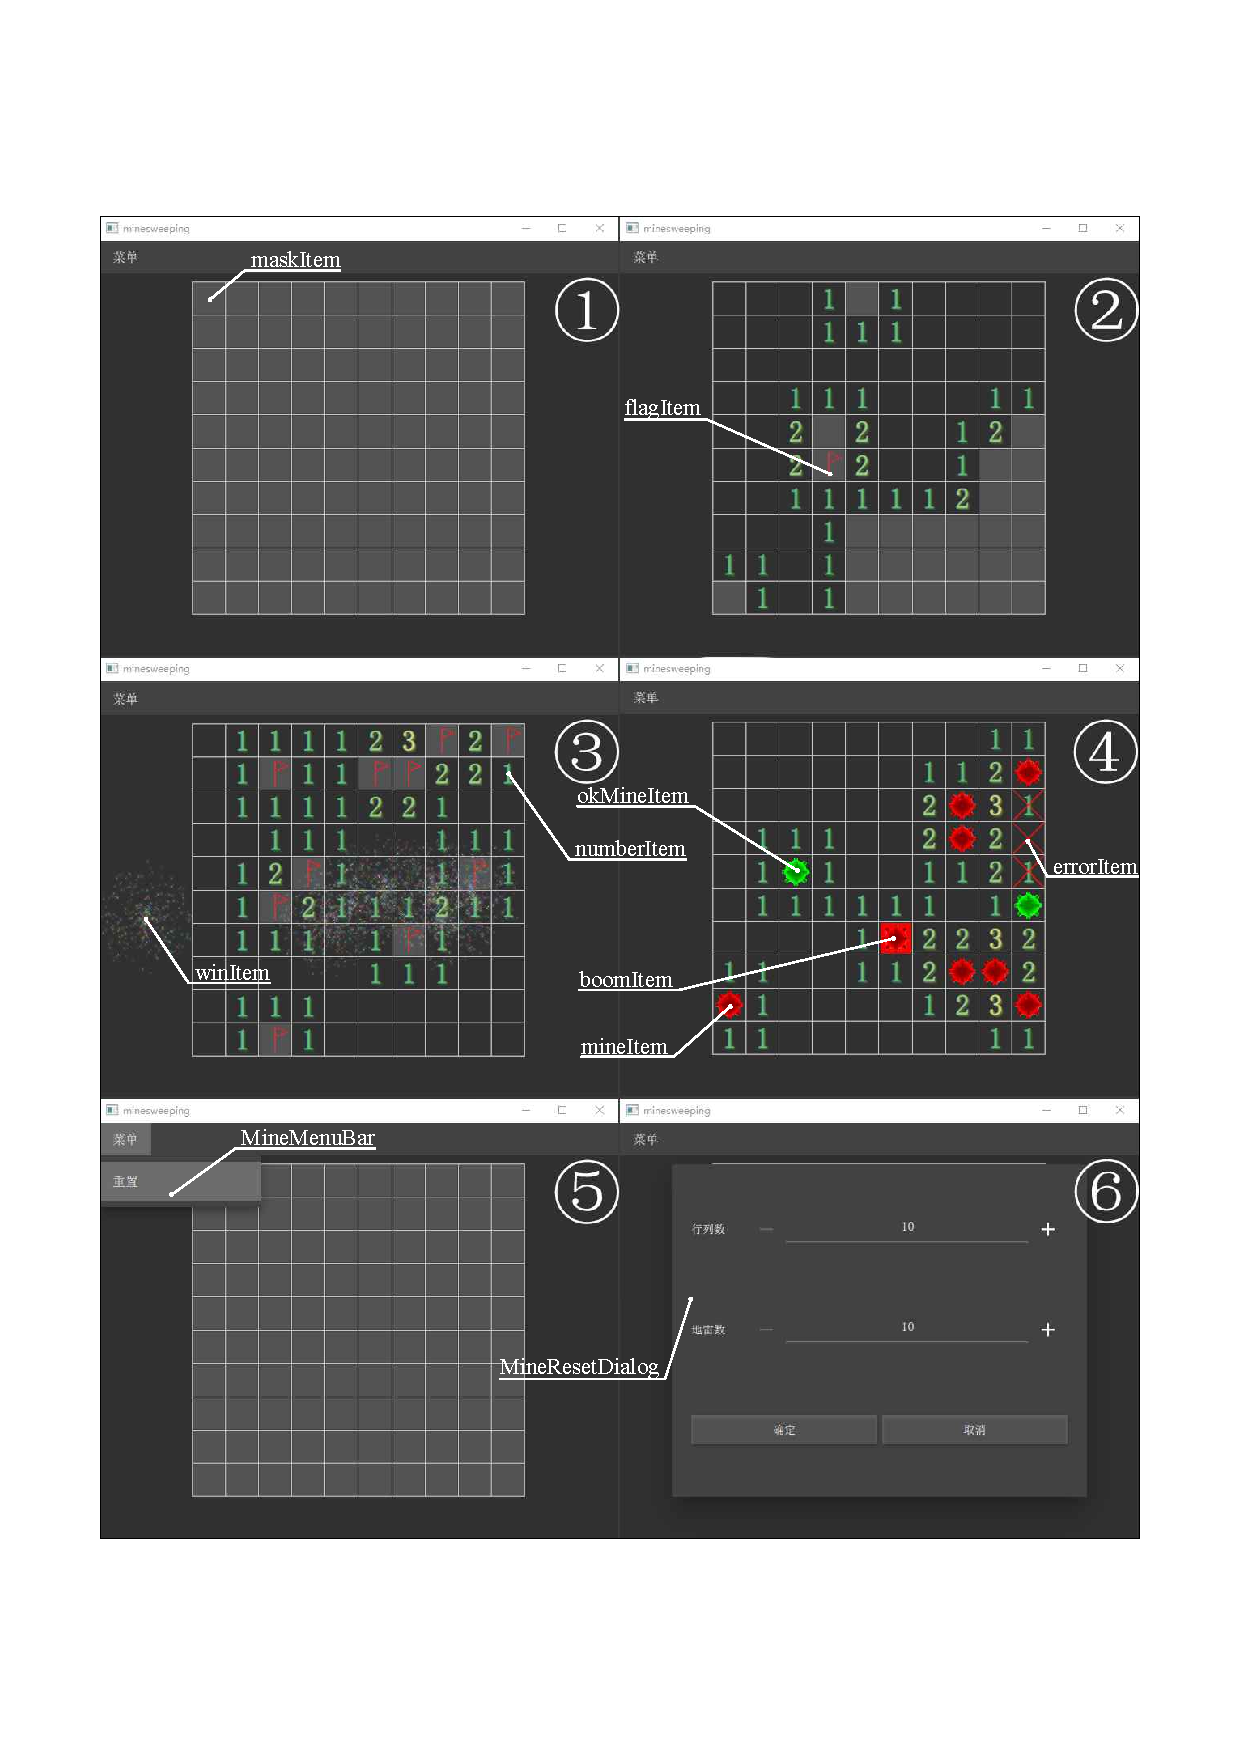
\includegraphics[width=0.95\textwidth]{chapter01/images/minesweeping_app.pdf} %图片路径
\caption{bigscene} %标题
\label{p000065} %索引
\end{figure}
%end图片


由于此章只是导引章节,
所以只列举“main.qml”源码。

%\begin{spacing}{1.0}
\refstepcounter{filesourcenumber}\label{f000083}    %增加源代码编号
\FloatBarrier                                  %强制完成浮动体布局
\begin{thebookfilesourceone}[escapeinside={(*@}{@*)},
caption=GoodLuck,
title=\filesourcenumbernameone \thefilesourcenumber
]
/*minesweeping/main.qml*/
import QtQuick 2.9
import sstd.minesweeping 1.0
import QtQuick.Controls 2.12

Pane {

    id : idRootOfMine

    padding: 0
    topInset: 0
    leftInset: 0
    rightInset: 0
    bottomInset: 0

    width: 640;
    height: 480;

    MineResetDialog{/*重置对话框*/
        id: idResetActionDialog ;
        onResizeMine : {
            idMineSweeping.setSizeScene(
                        rowAndColumn,
                        rowAndColumn,
                        mineSize);
        }
    }

    MineMenuBar{/*菜单*/
        id : idMenuBar
        width: parent.width ;
        anchors.top: parent.top ;
        anchors.left: parent.left ;
        onToResetAction: {
            idResetActionDialog.open() ;
        }
    }

    MineSweeping{

        id : idMineSweeping

        anchors.centerIn: parent;
        property double minWidthHeight:
            Math.min( parent.height , parent.width );
        width: minWidthHeight * 0.8;
        height: minWidthHeight * 0.8;

        maskItem : Rectangle {/*遮罩*/
            anchors.centerIn: parent       ;
            width: parent.width * 0.95     ;
            height: parent.height * 0.95   ;
            color: Qt.rgba( 0.45,0.46,0.47,0.5 ) ;
            Behavior on opacity{
                NumberAnimation{
                    duration: 333
                }
            }
            Behavior on width{
                NumberAnimation{
                    duration: 25
                }
            }
            Behavior on height{
                NumberAnimation{
                    duration: 25
                }
            }
        }

        flagItem : Flag{/*地雷标记*/
            anchors.centerIn: parent ;
            width  : parent.width * 0.75 ;
            height : parent.height * 0.75 ;
            Behavior on width{
                NumberAnimation{
                    duration: 33
                }
            }
            Behavior on height{
                NumberAnimation{
                    duration: 33
                }
            }
        }

        numberItem : Number{/*数字*/
            anchors.centerIn: parent ;
            width  : parent.width * 0.9 ;
            height : parent.height * 0.9 ;
            Behavior on width{
                NumberAnimation{
                    duration: 33
                }
            }
            Behavior on height{
                NumberAnimation{
                    duration: 33
                }
            }
        }

        errorItem : Error{/*识别错误标记*/
            anchors.centerIn: parent ;
            width  : parent.width * 0.9 ;
            height : parent.height * 0.9 ;
            Behavior on width{
                NumberAnimation{
                    duration: 33
                }
            }
            Behavior on height{
                NumberAnimation{
                    duration: 33
                }
            }
        }

        mineItem : Mine{/*未识别的地雷*/
            anchors.centerIn: parent ;
            width  : parent.width * 0.9 ;
            height : parent.height * 0.9 ;
            Behavior on width{
                NumberAnimation{
                    duration: 33
                }
            }
            Behavior on height{
                NumberAnimation{
                    duration: 33
                }
            }
        }

        okMineItem : OkMine{/*正确识别的地雷*/
            anchors.centerIn: parent ;
            width  : parent.width * 0.9 ;
            height : parent.height * 0.9 ;
            Behavior on width{
                NumberAnimation{
                    duration: 33
                }
            }
            Behavior on height{
                NumberAnimation{
                    duration: 33
                }
            }
        }

        boomItem : Boom {/*引爆的地雷*/
            anchors.centerIn: parent ;
            width  : parent.width * 0.9 ;
            height : parent.height * 0.9 ;
            Behavior on width{
                NumberAnimation{
                    duration: 33
                }
            }
            Behavior on height{
                NumberAnimation{
                    duration: 33
                }
            }
        }

        winItem : Win {/*游戏成功时显示*/
            anchors.centerIn: parent
            width:idRootOfMine.width * 0.85
            height:idRootOfMine.height
        }

    }

}/*~Pane*/(*@\marginpar[\hfill\setlength\fboxsep{2pt}\fbox{\footnotesize{\kaishu\parbox{1em}{\setlength{\baselineskip}{2pt}\filesourcenumbernameone}}\footnotesize{\thefilesourcenumber}}]{\setlength\fboxsep{2pt}\fbox{\footnotesize{\kaishu\parbox{1em}{\setlength{\baselineskip}{2pt}\filesourcenumbernameone}}\footnotesize{\thefilesourcenumber}}}@*)\end{thebookfilesourceone}          %抄录环境
\addtocounter{lstlisting}{-1}   %sub lstlisting counter ...
%\end{spacing}


从\filesourcenumbernameone\ \ref{f000083}可
以看出,
QML轻松的将一个大型复杂整体
轻松地
分割成了一个个相对独立的小结构;
同时又
将一个个相对独立的小结构
毫无阻碍地
合成了一个大的整体。

结构、样式和逻辑
在不同粒度下都得到了有机的
分离与统一。



毫无疑问,恰如其名,Qt Quick将为现代通用GUI开发注入急速。


% ______all_key_words
% the_book_chapter the_book_subsection the_book_subsubsection
% the_book_section the_book_image the_book_table
% the_book_file the_book_tree_file the_book_command_file
% littlelongworld tabbing ref
% figurename tablename filesourcenumbernameone
% treeindexnumbernameone commandnumbernameone footnote
% item itemize comment textbullet
% \hspace*{\parindent}
% FloatBarrier







%使用XeLaTeX编译
%版权所有,翻版必究
%本文件由程序自动生成,任何修改将被覆盖
%2019 年 01 月 23 日



